\documentclass[11pt]{article}

% ── Packages ──────────────────────────────────────────────────────────────
\usepackage[margin=1in]{geometry}
\usepackage{amsmath,amssymb,amsthm}
\usepackage{hyperref}
\usepackage{cleveref}
\usepackage{listings}
\usepackage{titlesec}
\usepackage{enumitem}
\usepackage{booktabs}
\usepackage{xcolor}
\usepackage{tikz}
\usetikzlibrary{arrows.meta,positioning,chains}

% ── Theorem Environments ──────────────────────────────────────────────────
\newtheorem{theorem}{Theorem}[section]
\newtheorem{lemma}[theorem]{Lemma}
\newtheorem{corollary}[theorem]{Corollary}
\newtheorem{proposition}[theorem]{Proposition}
\newtheorem{definition}[theorem]{Definition}
\newtheorem{remark}[theorem]{Remark}
\newtheorem{example}[theorem]{Example}
\newtheorem{axiom}{Axiom}

% ── Listings ──────────────────────────────────────────────────────────────
\definecolor{codebg}{HTML}{F5F5F5}
\definecolor{codegreen}{HTML}{2E7D32}
\definecolor{codeblue}{HTML}{1565C0}
\definecolor{codegray}{HTML}{757575}
\definecolor{codepurple}{HTML}{7B1FA2}

\lstdefinelanguage{JAPL}{
  keywords={fn, let, mut, type, effect, handle, match, with, where, impl, trait, struct, enum, pub, mod, use, return, if, else, for, in, do, spawn, supervise, derive, async, await, move, ref, self, Self, true, false},
  keywordstyle=\color{codeblue}\bfseries,
  ndkeywords={Int, String, Bool, Option, Result, IO, Process, List, Vec, Unit, Never, Owned, Ref, MutRef},
  ndkeywordstyle=\color{codepurple}\bfseries,
  comment=[l]{//},
  morecomment=[s]{/*}{*/},
  commentstyle=\color{codegray}\itshape,
  stringstyle=\color{codegreen},
  morestring=[b]",
  sensitive=true,
}

\lstset{
  language=JAPL,
  backgroundcolor=\color{codebg},
  basicstyle=\ttfamily\small,
  breaklines=true,
  frame=single,
  rulecolor=\color{codegray},
  numbers=left,
  numberstyle=\tiny\color{codegray},
  tabsize=2,
  captionpos=b,
  aboveskip=1em,
  belowskip=1em,
}

% ── Macros ────────────────────────────────────────────────────────────────
\newcommand{\DP}{\mathcal{D}(P)}
\newcommand{\CP}{\mathcal{C}(P)}
\newcommand{\RP}{\mathcal{R}(P)}
\newcommand{\witness}{w_d}
\newcommand{\omegadata}{\omega\text{-data}}
\newcommand{\Cat}{\mathbf{Cat}}
\newcommand{\Set}{\mathbf{Set}}
\newcommand{\Cop}{\mathcal{C}^{\mathrm{op}}}
\newcommand{\Nat}{\mathrm{Nat}}
\newcommand{\id}{\mathrm{id}}

% ── Title ─────────────────────────────────────────────────────────────────
\title{\textbf{The Minimal Runtime Axiom} \\[0.5em]
  \large Runtime Is Proof of Ignorance: \\
  A Type-Theoretic and Category-Theoretic Formalization \\
  of the Compile-Time/Runtime Boundary}

\author{
  Matthew Long \\
  \textit{The YonedaAI Collaboration} \\
  \textit{YonedaAI Research Collective} \\
  Chicago, IL \\
  \texttt{matthew@yonedaai.com}
}

\date{March 2026}

\begin{document}
\maketitle

% ══════════════════════════════════════════════════════════════════════════
% ABSTRACT
% ══════════════════════════════════════════════════════════════════════════
\begin{abstract}
We formalize the principle that \emph{runtime is proof of ignorance}: every decision
that a program defers to runtime exists precisely because the type system---or more
broadly, the static reasoning apparatus---failed to capture it at compile time. We
introduce the \textbf{Minimal Runtime Axiom}, which states that the runtime decision
set of a program $P$ is exactly the complement of the compile-time decidable set:
$\RP = \DP \setminus \CP$, where $\CP$ consists of all decisions admitting a
\emph{static witness} $\witness = (\tau, \pi, \sigma)$---a type $\tau$, a proof term
$\pi$ inhabiting that type, and a staging certificate $\sigma$ guaranteeing that $\pi$
is constructible before execution. We derive three corollaries: (1)~\textbf{Runtime
Irreducibility}---a decision is legitimately runtime if and only if it depends on
$\omegadata$ (user input, I/O, time, nondeterminism); (2)~\textbf{The Duality}---the
cardinality of the runtime set is proportional to the epistemic deficit of the type
system; (3)~\textbf{The Yoneda Correspondence}---runtime type inspection is isomorphic
to failure of the Yoneda embedding. We develop the full category-theoretic treatment,
demonstrate applications to language design through the JAPL programming language, and
characterize the impossibility boundary imposed by $\omegadata$ through connections to
the halting problem and Rice's theorem. The axiom provides language designers with a
precise criterion: \emph{every non-$\omega$ decision at runtime is a theorem waiting
to be proven}.
\end{abstract}

\tableofcontents
\newpage

% ══════════════════════════════════════════════════════════════════════════
% 1. INTRODUCTION
% ══════════════════════════════════════════════════════════════════════════
\section{Introduction}
\label{sec:introduction}

The history of programming language design is, in large part, the history of moving
decisions from runtime to compile time. This transfer has been the central animating
force behind type systems, static analysis, formal verification, and the entire
enterprise of programming language theory.

In the earliest days of computing, \emph{everything} was a runtime decision. Assembly
language programs performed all type dispatch, memory management, error handling, and
protocol negotiation dynamically. The machine had no opinion about the meaning of a
bit pattern; that was the programmer's responsibility, enforced only by hope and
documentation.

The introduction of high-level languages began the great migration. FORTRAN moved
numeric type dispatch to compile time. C moved function signatures and basic type
compatibility. ML and Haskell moved parametric polymorphism, algebraic data type
exhaustiveness, and many forms of error handling. Rust moved memory management, data
race prevention, and lifetime reasoning. Dependent type systems in Idris, Agda, and
Lean moved array bounds checking, protocol adherence, and arithmetic invariants.

Each of these advances can be understood as a single motion: the construction of a
\emph{static witness} that renders a runtime check unnecessary. When ML's type checker
proves that a function application is well-typed, it has constructed a witness that
eliminates the need for runtime type dispatch. When Rust's borrow checker proves that
references do not outlive their referents, it has constructed a witness that eliminates
the need for garbage collection or manual deallocation.

This paper formalizes this observation as the \textbf{Minimal Runtime Axiom}: the
runtime decision set of any program is exactly the set of decisions for which no
static witness can be constructed. We develop the formal apparatus---decision spaces,
static witnesses, staging certificates---and derive three corollaries that characterize
the nature of runtime, the relationship between type system expressiveness and runtime
overhead, and the categorical structure underlying the compile-time/runtime boundary.

The axiom is not a theorem in the traditional sense; it is a \emph{design principle},
akin to the Church-Turing thesis. It cannot be proven from more primitive axioms
because it defines what we \emph{mean} by optimal language design. But like the
Church-Turing thesis, it unifies a vast body of existing work under a single principle
and provides a generative framework for future research.

We organize the paper as follows. \Cref{sec:decision-space} defines the decision
space of a program. \Cref{sec:axiom} states the axiom formally. \Cref{sec:witnesses}
develops the theory of static witnesses. \Cref{sec:corollary1,sec:corollary2,sec:corollary3}
present the three corollaries. \Cref{sec:hierarchy} describes the decision transfer
hierarchy. \Cref{sec:language-design,sec:agent-arch} apply the axiom to language
design and agent architecture. \Cref{sec:related} surveys related work.
\Cref{sec:impossibility} characterizes the impossibility boundary.
\Cref{sec:category-theory} develops the full categorical formalization.
\Cref{sec:conclusion} concludes.


% ══════════════════════════════════════════════════════════════════════════
% 2. THE DECISION SPACE OF A PROGRAM
% ══════════════════════════════════════════════════════════════════════════
\section{The Decision Space of a Program}
\label{sec:decision-space}

\begin{definition}[Decision]
\label{def:decision}
A \emph{decision} $d$ in a program $P$ is any point in the execution where the
program's behavior depends on a choice among alternatives. Formally, $d$ is a
function $d : \Sigma \to A$ from the program state space $\Sigma$ to an action
space $A$ with $|A| \geq 2$.
\end{definition}

\begin{definition}[Decision Space]
\label{def:decision-space}
The \emph{decision space} $\DP$ of a program $P$ is the set of all decisions
that must be resolved during the lifecycle of $P$:
\[
  \DP = \{ d_1, d_2, \ldots, d_n \}
\]
where each $d_i$ is a decision as defined above.
\end{definition}

The decision space encompasses a remarkably wide range of program behaviors. We
categorize the most significant classes:

\paragraph{Type Dispatch.}
When a program must determine the concrete type of a value to select behavior---e.g.,
virtual method dispatch, pattern matching on variants, \texttt{instanceof} checks---each
such point constitutes a decision.

\paragraph{Memory Layout and Lifetime.}
When to allocate, where to allocate (stack vs.\ heap), when to deallocate, and how to
manage shared references are all decisions. In C, most of these are runtime. In Rust,
most are compile-time.

\paragraph{Null and Option Handling.}
Every nullable reference introduces a decision: is this reference null? Languages with
\texttt{Option<T>} and exhaustive pattern matching transfer this decision to compile time.

\paragraph{Bounds Checking.}
Array access $a[i]$ introduces the decision: is $i$ within bounds? In most languages
this is runtime. With dependent types, it can be compile-time:

\begin{lstlisting}[caption={Bounds checking as a compile-time decision in JAPL}]
fn safe_index<N: Nat>(arr: Vec<T, N>, i: Fin<N>) -> T {
  // No bounds check needed: i : Fin<N> is a proof that i < N
  arr.get_unchecked(i)
}
\end{lstlisting}

\paragraph{Protocol Compatibility.}
Network protocols, API contracts, and serialization formats all involve decisions about
compatibility. Session types transfer these to compile time.

\paragraph{Resource Lifetime.}
File handles, network connections, database transactions---when to acquire and release
resources involves decisions that linear types can capture statically.

\paragraph{Effect Handling.}
Whether a function performs I/O, throws exceptions, spawns threads, or allocates memory
are decisions that effect systems transfer to compile time.

\begin{definition}[$\omega$-Dependent and $\omega$-Independent Decisions]
\label{def:omega}
A decision $d \in \DP$ is \emph{$\omega$-dependent} if it depends on data not
available until runtime: user input, I/O results, sensor data, current time, or
nondeterministic choice. Otherwise, $d$ is \emph{$\omega$-independent}.
\end{definition}

\begin{remark}
The distinction between $\omega$-dependent and $\omega$-independent decisions is the
fundamental partition of $\DP$. As we shall see, $\omega$-independent decisions are
precisely those that \emph{could}, in principle, be transferred to compile time.
\end{remark}

\begin{example}[Decision Space of a Web Server]
Consider a web server program $P_{\text{web}}$. Its decision space includes:
\begin{itemize}[nosep]
  \item \textbf{$\omega$-dependent}: Which URL is requested? What are the request headers? What is the database state?
  \item \textbf{$\omega$-independent}: Is the URL handler well-typed? Are all database queries type-safe? Will the response be properly serialized? Are resources properly released?
\end{itemize}
A language satisfying the Minimal Runtime Axiom would transfer \emph{all} $\omega$-independent decisions to compile time, leaving only the genuinely dynamic decisions at runtime.
\end{example}


% ══════════════════════════════════════════════════════════════════════════
% 3. THE AXIOM: COMPILE-TIME SUPREMACY
% ══════════════════════════════════════════════════════════════════════════
\section{The Axiom: Compile-Time Supremacy}
\label{sec:axiom}

We now state the central principle of this paper.

\begin{axiom}[The Minimal Runtime Axiom]
\label{axiom:mra}
For any program $P$, the \emph{minimal runtime decision set} is:
\[
  \RP = \DP \setminus \CP
\]
where $\CP = \{ d \in \DP \mid \exists\, \witness = (\tau, \pi, \sigma) \}$ is the
set of decisions admitting a static witness. A language design is \emph{optimal with
respect to the axiom} if no decision in $\RP$ admits a static witness---that is, if
every decision remaining at runtime is genuinely irreducible.
\end{axiom}

Several aspects of this formulation deserve comment.

\paragraph{Why ``Axiom'' and Not ``Theorem''?}
The Minimal Runtime Axiom is not derivable from more primitive principles. It is a
\emph{design principle}---a statement about what we believe optimal language design
should achieve. In this respect, it is analogous to the Church-Turing thesis: it
cannot be proven, but it can be supported by evidence, and it can be used generatively
to discover new static analysis techniques.

\paragraph{The Residual Set.}
The set $\RP$ represents the \emph{irreducible runtime core} of a program. For any
fixed type system, $\CP$ is determined, and hence $\RP$ is determined. But as type
systems grow more expressive, $\CP$ grows, and $\RP$ shrinks. The axiom asserts that
the ideal endpoint is the minimum possible $\RP$---which, as we show in
\Cref{sec:corollary1}, consists exactly of $\omega$-dependent decisions.

\paragraph{The Pragmatic Dimension.}
In practice, language designers must balance expressiveness against complexity.
Dependent type systems can transfer more decisions to compile time than simple type
systems, but at the cost of more complex type annotations and proof obligations. The
axiom does not mandate dependent types; it provides a \emph{metric} for evaluating
language design choices. Each decision remaining at runtime should be justified: either
it is genuinely $\omega$-dependent, or it is a deliberate trade-off between type system
complexity and runtime cost.

\begin{remark}[The Economy of Ignorance]
\label{rem:economy}
The axiom as stated is a \emph{normative ideal}, not a pragmatic mandate. In practice,
constructing a static witness $\witness$ incurs a \emph{proof burden}---the human effort
to encode invariants as types and supply proof terms. When the cost of constructing
$\witness$ exceeds the cost of the runtime check it eliminates, a rational language
designer may choose to leave the decision at runtime. We call this the \emph{economy of
ignorance}: sometimes it is cheaper to be ignorant. The axiom remains valuable as a
metric---it tells us \emph{what} we are paying for and \emph{why}---even when full
optimization is impractical. The pragmatic version of the axiom is: \emph{every
non-$\omega$ decision at runtime should be a conscious, costed trade-off, not an
accidental oversight}.
\end{remark}

\begin{proposition}[Monotonicity]
\label{prop:monotone}
If type system $T_1$ is strictly more expressive than type system $T_2$ (i.e.,
$\mathcal{C}_{T_2}(P) \subset \mathcal{C}_{T_1}(P)$ for all $P$), then
$\mathcal{R}_{T_1}(P) \subset \mathcal{R}_{T_2}(P)$ for all $P$. More expressive
type systems yield smaller runtime sets.
\end{proposition}

\begin{proof}
By set complementation: if $\mathcal{C}_{T_2}(P) \subset \mathcal{C}_{T_1}(P)$,
then $\DP \setminus \mathcal{C}_{T_1}(P) \subset \DP \setminus \mathcal{C}_{T_2}(P)$.
\end{proof}


% ══════════════════════════════════════════════════════════════════════════
% 4. STATIC WITNESSES
% ══════════════════════════════════════════════════════════════════════════
\section{Static Witnesses}
\label{sec:witnesses}

The notion of a static witness is the technical core of the axiom. We develop it in
detail.

\begin{definition}[Static Witness]
\label{def:witness}
A \emph{static witness} for a decision $d \in \DP$ is a triple $\witness = (\tau, \pi, \sigma)$
where:
\begin{enumerate}[nosep]
  \item $\tau$ is a \emph{type} that encodes the invariant making $d$ unnecessary---that is,
        $\tau$ expresses the property that, if established, determines $d$'s outcome without
        runtime inspection.
  \item $\pi$ is a \emph{proof term} (an inhabitant of $\tau$)---a concrete construction
        demonstrating that the invariant holds.
  \item $\sigma$ is a \emph{staging certificate}---evidence that $\pi$ can be constructed
        \emph{before execution}, i.e., at compile time, type-check time, or proof time.
        Formally, in the framework of modal logic for staged computation~\cite{davies2001modal},
        $\sigma$ witnesses that $\pi$ inhabits a type of the form $\Box\,\tau$ (the modal
        necessity operator), indicating that $\pi$ is available at \emph{all} future stages,
        having been constructed at the current (pre-execution) stage. In multi-stage
        programming systems like MetaOCaml, $\sigma$ corresponds to the absence of
        \texttt{Ref} (cross-stage persistence of mutable state) in the proof term---i.e.,
        $\pi$ is a \emph{closed} term at stage 0.
\end{enumerate}
\end{definition}

The three components serve distinct purposes. The type $\tau$ defines \emph{what} must
be proven. The proof term $\pi$ demonstrates \emph{that} it holds. The staging
certificate $\sigma$ guarantees \emph{when} the proof is available---specifically, that
$\pi$ is constructible in a phase prior to execution, formalized through the modal
$\Box$ operator of S4 logic applied to the staging hierarchy. Without $\sigma$,
we might have a proof that can only be constructed at runtime (e.g., a dynamic check),
which does not eliminate the runtime decision.

We now present five central examples of static witnesses.

\subsection{Type Safety}

\begin{example}[Well-Typed Programs Don't Go Wrong]
\label{ex:type-safety}
Consider the decision ``does this function application have the correct argument type?''
\begin{align*}
  \tau &= \Gamma \vdash e_1\,e_2 : B \quad\text{(the typing judgment)} \\
  \pi &= \text{the type derivation tree} \\
  \sigma &= \text{the type checker terminates at compile time}
\end{align*}
Milner's slogan ``well-typed programs don't go wrong'' is precisely the statement that
this witness eliminates the need for runtime type checks.
\end{example}

\subsection{Null Safety}

\begin{example}[Option Types as Static Witnesses]
\label{ex:null-safety}
Consider the decision ``is this reference null?''
\begin{align*}
  \tau &= \texttt{Option<T>} \text{ with exhaustive pattern matching} \\
  \pi &= \text{exhaustiveness proof from the match checker} \\
  \sigma &= \text{match exhaustiveness is checked at compile time}
\end{align*}
In JAPL, the witness is constructed as follows:
\end{example}

\begin{lstlisting}[caption={Null safety through exhaustive matching in JAPL}]
fn process(value: Option<Config>) -> Result<Output, Error> {
  match value {
    Some(config) => Ok(compute(config)),
    None => Err(Error::MissingConfig),
  }
  // Exhaustiveness checked at compile time.
  // No null pointer exception possible.
}
\end{lstlisting}

\subsection{Memory Safety}

\begin{example}[Ownership as Static Witness]
\label{ex:memory-safety}
Consider the decision ``when should this memory be freed?''
\begin{align*}
  \tau &= \text{linear type / ownership type} \\
  \pi &= \text{proof that each value has exactly one owner} \\
  \sigma &= \text{the borrow checker runs at compile time}
\end{align*}
\end{example}

\begin{lstlisting}[caption={Memory safety through ownership in JAPL}]
fn transfer(data: Owned<Buffer>) -> Owned<Buffer> {
  // data is moved here; original binding is invalidated.
  // Compile-time guarantee: no double-free, no use-after-free.
  let processed = transform(data);  // Ownership transferred
  processed  // Ownership returned to caller
}
\end{lstlisting}

\subsection{Effect Safety}

\begin{example}[Effect Types as Static Witnesses]
\label{ex:effect-safety}
Consider the decision ``does this function perform I/O?''
\begin{align*}
  \tau &= \text{effect row, e.g., } \texttt{fn() -> T / \{IO, Async\}} \\
  \pi &= \text{effect inference derivation} \\
  \sigma &= \text{effect checking at compile time}
\end{align*}
\end{example}

\begin{lstlisting}[caption={Effect safety through effect types in JAPL}]
effect FileSystem {
  fn read_file(path: String) -> Result<String, IOError>
  fn write_file(path: String, content: String) -> Result<(), IOError>
}

// The effect annotation is the static witness:
// this function's side effects are fully captured at compile time.
fn process_data() -> Result<Report, Error> / {FileSystem, Log} {
  let raw = do FileSystem.read_file("data.csv")?;
  let report = analyze(raw);  // pure: no effect annotation needed
  do Log.info("Report generated");
  Ok(report)
}
\end{lstlisting}

\subsection{Protocol Safety}

\begin{example}[Session Types as Static Witnesses]
\label{ex:protocol-safety}
Consider the decision ``is this protocol message sent in the correct order?''
\begin{align*}
  \tau &= \text{session type, e.g., } \texttt{!Request.?Response.End} \\
  \pi &= \text{session type derivation showing protocol adherence} \\
  \sigma &= \text{session type checking at compile time}
\end{align*}
\end{example}

\begin{lstlisting}[caption={Protocol safety through session types in JAPL}]
type ClientProtocol = Send<Request> >> Recv<Response> >> Close;

fn client(channel: Channel<ClientProtocol>) -> Result<Response, Error> {
  let channel = channel.send(Request::new("query"))?;
  let (response, channel) = channel.recv()?;
  channel.close();
  // Protocol adherence proven at compile time.
  // Out-of-order messages are type errors, not runtime errors.
  Ok(response)
}
\end{lstlisting}

\begin{theorem}[Witness Compositionality]
\label{thm:compositionality}
If decisions $d_1$ and $d_2$ have static witnesses $w_{d_1} = (\tau_1, \pi_1, \sigma_1)$
and $w_{d_2} = (\tau_2, \pi_2, \sigma_2)$, then the compound decision $d_1 \wedge d_2$
has static witness $w_{d_1 \wedge d_2} = (\tau_1 \times \tau_2, (\pi_1, \pi_2), \sigma_1 \wedge \sigma_2)$.
\end{theorem}

\begin{proof}
The product type $\tau_1 \times \tau_2$ encodes both invariants simultaneously. The
pair $(\pi_1, \pi_2)$ inhabits $\tau_1 \times \tau_2$ (by the introduction rule for
product types). The compound staging certificate $\sigma_1 \wedge \sigma_2$ holds if
both $\pi_1$ and $\pi_2$ are constructible before execution, which obtains by
assumption. Thus $w_{d_1 \wedge d_2}$ satisfies \Cref{def:witness}.
\end{proof}


% ══════════════════════════════════════════════════════════════════════════
% 5. COROLLARY 1: RUNTIME IRREDUCIBILITY
% ══════════════════════════════════════════════════════════════════════════
\section{Corollary 1: Runtime Irreducibility}
\label{sec:corollary1}

\begin{definition}[$\omega$-Data]
\label{def:omega-data}
The \emph{$\omega$-data} of a program execution is the totality of information that is
not available at any pre-execution phase:
\begin{enumerate}[nosep]
  \item \textbf{User input}: keystrokes, mouse events, API requests
  \item \textbf{I/O results}: file contents, network responses, database query results
  \item \textbf{Temporal data}: current time, elapsed durations, timeouts
  \item \textbf{Nondeterminism}: random number generation, thread scheduling, hardware interrupts
  \item \textbf{Environmental state}: available memory, CPU load, network latency
\end{enumerate}
We denote the $\omega$-data of an execution as $\omega$.
\end{definition}

\begin{corollary}[Runtime Irreducibility]
\label{cor:irreducibility}
A decision $d \in \DP$ is \emph{legitimately runtime} (i.e., no static witness can
exist for $d$) if and only if $d$ depends on $\omegadata$. Formally:
\[
  d \in \RP_{\min} \iff d = f(\omega) \text{ for some non-trivial } f
\]
where $\RP_{\min}$ is the minimal possible runtime set (under an arbitrarily powerful
type system) and $f$ is non-trivial in the sense that different values of $\omega$
yield different decisions.
\end{corollary}

\begin{proof}
($\Rightarrow$) Suppose $d$ does not depend on $\omegadata$. Then $d$ is fully
determined by the program text $P$ and the compile-time environment. In a sufficiently
expressive type system (e.g., the Calculus of Constructions with induction), we can
encode this determination as a type $\tau$, construct the proof term $\pi$ at type-check
time, and the staging certificate $\sigma$ is immediate. Thus $d \in \CP$ and
$d \notin \RP_{\min}$.

($\Leftarrow$) Suppose $d$ depends on $\omegadata$, i.e., $d = f(\omega)$ for
non-trivial $f$. By definition, $\omega$ is not available before execution. Any proof
term $\pi$ for $\tau$ encoding $d$'s outcome would need to reference $\omega$, but
the staging certificate $\sigma$ requires $\pi$ to be constructible before execution.
Since $\omega$ is unavailable pre-execution, no such $\sigma$ can exist. Thus
$d \notin \CP$ and $d \in \RP_{\min}$.
\end{proof}

\begin{example}[False Runtime: Decisions Masquerading as $\omega$-Dependent]
\label{ex:false-runtime}
Many decisions that \emph{appear} to require runtime resolution are actually
$\omega$-independent:

\begin{enumerate}[nosep]
  \item \textbf{Virtual dispatch} on a closed type hierarchy: the set of possible
    types is known at compile time; with whole-program analysis or sealed traits,
    dispatch can be monomorphized.

  \item \textbf{Null checks} on values that were already validated: with flow-sensitive
    typing or refinement types, the non-null invariant can be tracked.

  \item \textbf{Array bounds checks} with statically known indices: with dependent
    types, the check is compiled away.

  \item \textbf{Serialization format negotiation} when both sides are compiled together:
    with type-derived codecs, the format is determined at compile time.

  \item \textbf{Garbage collection} pauses: with linear or affine types, memory
    lifetime is statically determined and no GC is needed.
\end{enumerate}
Each of these is a decision currently at runtime in mainstream languages that a more
expressive type system could transfer to compile time.
\end{example}

\begin{remark}
The Runtime Irreducibility corollary provides a precise criterion for evaluating
language features: every runtime decision should be tested against the question ``does
this genuinely depend on $\omegadata$?'' If not, it is a candidate for static
elimination.
\end{remark}


% ══════════════════════════════════════════════════════════════════════════
% 6. COROLLARY 2: THE DUALITY
% ══════════════════════════════════════════════════════════════════════════
\section{Corollary 2: The Duality}
\label{sec:corollary2}

\begin{corollary}[The Duality]
\label{cor:duality}
For a program $P$ under type system $T$:
\[
  |\mathcal{R}_T(P)| = |\DP| - |\mathcal{C}_T(P)| \propto \text{epistemic deficit of } T
\]
The number of runtime decisions is directly proportional to the \emph{epistemic deficit}
of the type system---the gap between what the type system \emph{can} express and what
\emph{could} in principle be expressed.
\end{corollary}

This corollary transforms the abstract axiom into a concrete tool for language
comparison. We map specific runtime mechanisms to their compile-time counterparts,
showing each as a decision transfer:

\begin{table}[h]
\centering
\caption{The Decision Transfer Map}
\label{tab:transfer-map}
\begin{tabular}{@{}lll@{}}
\toprule
\textbf{Runtime Mechanism} & \textbf{Compile-Time Transfer} & \textbf{Witness Type} \\
\midrule
Dynamic dispatch      & Monomorphization / Type classes  & Type instantiation \\
Null pointer checks   & Option types + exhaustiveness    & Pattern completeness \\
Array bounds checks   & Dependent types / Fin<N>         & Arithmetic proof \\
Garbage collection    & Linear / affine types            & Ownership proof \\
Exception handling    & Result types + propagation       & Error type tracking \\
Serialization         & Type-derived codecs              & Schema derivation \\
Dynamic linking       & Whole-program compilation        & Link-time resolution \\
Reflection            & Type classes / higher-kinded     & Yoneda embedding \\
Runtime casts         & Generalized algebraic data types & Type equality witness \\
Capability checks     & Effect types / permission types  & Capability proof \\
\bottomrule
\end{tabular}
\end{table}

We elaborate on several of these transfers.

\subsection{Dynamic Dispatch to Monomorphization}

In languages with subtype polymorphism (Java, C++, Python), method calls on
polymorphic types require virtual dispatch tables consulted at runtime. The decision
``which implementation to call'' is deferred to runtime.

With parametric polymorphism and monomorphization (as in Rust and JAPL), the compiler
specializes generic functions for each concrete type argument, resolving dispatch at
compile time:

\begin{lstlisting}[caption={Monomorphization eliminates runtime dispatch in JAPL}]
trait Serialize {
  fn to_bytes(self: Ref<Self>) -> Vec<u8>;
}

// Monomorphized: separate compiled code for each T
fn send_message<T: Serialize>(msg: Ref<T>) -> Result<(), NetError> / {Network} {
  let bytes = msg.to_bytes();  // Static dispatch, no vtable
  do Network.send(bytes)
}
\end{lstlisting}

\subsection{Garbage Collection to Ownership}

Garbage collection is a runtime mechanism for the decision ``when should this memory
be freed?'' With linear types:

\begin{lstlisting}[caption={Ownership eliminates garbage collection in JAPL}]
fn pipeline() -> Result<Report, Error> {
  let data = Owned::new(load_data()); // Allocated
  let processed = transform(data);     // data moved, original dropped
  let report = summarize(processed);   // processed moved, original dropped
  report // Returned to caller; caller owns it
  // All memory freed deterministically at scope boundaries.
  // No GC pauses. No reference counting overhead.
}
\end{lstlisting}

\subsection{Exception Handling to Result Types}

Exceptions make error propagation invisible: any function might throw, and the decision
``will this function raise an exception?'' is runtime. Result types transfer this:

\begin{lstlisting}[caption={Result types transfer error decisions to compile time in JAPL}]
fn parse_config(path: String) -> Result<Config, ConfigError> / {FileSystem} {
  let content = do FileSystem.read_file(path)
    .map_err(ConfigError::IoError)?;
  let config = parse_toml(content)
    .map_err(ConfigError::ParseError)?;
  validate(config)
    .map_err(ConfigError::ValidationError)
  // Every error path is visible in the type.
  // The caller MUST handle all three error variants.
}
\end{lstlisting}

\begin{theorem}[Duality Ordering]
\label{thm:ordering}
The decision transfer map induces a partial order on type systems. For type systems
$T_1, T_2$:
\[
  T_1 \preceq T_2 \iff \forall P.\; \mathcal{C}_{T_1}(P) \subseteq \mathcal{C}_{T_2}(P)
\]
This order has the simply-typed lambda calculus near the bottom and the Calculus of
Inductive Constructions near the top.
\end{theorem}

\begin{proof}
The relation $\preceq$ is clearly reflexive and transitive. Antisymmetry holds up to
equivalence of type systems (systems that accept the same programs with the same
static guarantees). The simply-typed lambda calculus provides witnesses only for basic
type safety. Each extension (polymorphism, algebraic types, linear types, dependent
types, etc.) strictly increases $\mathcal{C}_T(P)$. The Calculus of Inductive
Constructions, being a full proof system, can in principle construct witnesses for all
$\omega$-independent decisions.
\end{proof}


% ══════════════════════════════════════════════════════════════════════════
% 7. COROLLARY 3: THE YONEDA CORRESPONDENCE
% ══════════════════════════════════════════════════════════════════════════
\section{Corollary 3: The Yoneda Correspondence}
\label{sec:corollary3}

The third corollary connects the axiom to category theory via the Yoneda lemma,
providing the deepest structural insight.

\begin{definition}[The Yoneda Embedding]
\label{def:yoneda}
For a locally small category $\mathcal{C}$, the \emph{Yoneda embedding} is the functor
$\mathsf{y} : \mathcal{C} \to [\Cop, \Set]$ defined by:
\[
  \mathsf{y}(A) = \mathrm{Hom}_{\mathcal{C}}(-, A)
\]
The Yoneda lemma states that for any presheaf $F : \Cop \to \Set$:
\[
  \Nat(\mathrm{Hom}_{\mathcal{C}}(-, A), F) \cong F(A)
\]
That is, an object $A$ is fully determined (up to isomorphism) by its relationships
with all other objects---its ``web of morphisms.''
\end{definition}

\begin{corollary}[The Yoneda Correspondence]
\label{cor:yoneda}
Runtime type inspection (reflection, \texttt{instanceof}, \texttt{typeof}, dynamic
casts) is isomorphic to failure of the Yoneda embedding in the type-theoretic category.
Formally, if a value $v$ of type $A$ is fully characterized by the morphisms
$\mathrm{Hom}(-, A)$ (i.e., by how it interacts with all other types via the type system),
then no runtime inspection of $v$ is necessary.
\end{corollary}

\begin{proof}
Let $\mathcal{C}_T$ be the category whose objects are types in type system $T$ and
whose morphisms are well-typed functions. The Yoneda embedding
$\mathsf{y} : \mathcal{C}_T \to [\mathcal{C}_T^{\mathrm{op}}, \Set]$ sends each
type $A$ to its representable presheaf $\mathrm{Hom}(-, A)$.

Suppose the Yoneda embedding is faithful for the relevant types---i.e., the type
system's morphisms (well-typed programs) fully characterize each type's behavior. Then
any property of a value $v : A$ that a runtime inspector could determine is already
determined by the morphisms involving $A$, which are precisely the well-typed programs
interacting with $v$. These morphisms are checked at compile time. Hence no runtime
inspection is needed.

Conversely, if runtime inspection \emph{is} needed for some property of $v : A$, then
that property is not captured by $\mathrm{Hom}(-, A)$---the Yoneda embedding fails to
distinguish $A$ from some other type $A'$ that differs in that property. This is
precisely a failure of the Yoneda embedding's faithfulness, meaning the type system has
insufficient morphisms to characterize the distinction.
\end{proof}

\begin{example}[Yoneda Failure in Java]
\label{ex:java-yoneda}
In Java, the \texttt{instanceof} operator is the canonical example of Yoneda failure.
Consider:
\begin{lstlisting}[language=Java, caption={Yoneda failure: runtime type inspection}]
void process(Object obj) {
    if (obj instanceof String) {
        // ...
    } else if (obj instanceof Integer) {
        // ...
    }
}
\end{lstlisting}
The type \texttt{Object} does not have enough morphisms (methods with specific type
signatures) to distinguish \texttt{String} from \texttt{Integer}. The Yoneda embedding
of \texttt{Object} conflates all subtypes, forcing runtime inspection.

In JAPL, this would be:
\begin{lstlisting}[caption={Yoneda success: compile-time type dispatch in JAPL}]
enum Value {
  Text(String),
  Number(Int),
}

fn process(v: Value) -> Output {
  match v {
    Value::Text(s)   => process_text(s),
    Value::Number(n) => process_number(n),
  }
  // Exhaustive match: the type Value has enough structure
  // (its Yoneda image is faithful) to resolve dispatch at compile time.
}
\end{lstlisting}
\end{example}

\begin{theorem}[Yoneda Completeness Criterion]
\label{thm:yoneda-complete}
A type system $T$ is \emph{Yoneda-complete} for a program $P$ if the Yoneda embedding
$\mathsf{y} : \mathcal{C}_T \to [\mathcal{C}_T^{\mathrm{op}}, \Set]$ is full and
faithful for all types occurring in $P$. In a Yoneda-complete type system, no runtime
type inspection is needed for $\omega$-independent decisions.
\end{theorem}

\begin{proof}
If $\mathsf{y}$ is full and faithful, then every natural transformation between
representable presheaves corresponds to a unique morphism in $\mathcal{C}_T$. This
means every ``testable relationship'' between types is captured by a compile-time
morphism (a well-typed function). Any decision that depends only on type relationships
(and not on $\omegadata$) can therefore be resolved by the type system.

Fullness ensures that every conceivable type relationship \emph{is} expressible as a
typed program. Faithfulness ensures that distinct type relationships remain
distinguishable. Together, they guarantee that the type system's view of the world is
as rich as the actual world of type relationships, leaving no room for runtime
discovery.
\end{proof}


% ══════════════════════════════════════════════════════════════════════════
% 8. THE DECISION TRANSFER HIERARCHY
% ══════════════════════════════════════════════════════════════════════════
\section{The Decision Transfer Hierarchy}
\label{sec:hierarchy}

The compile-time/runtime boundary is not binary. There is a hierarchy of stages at
which decisions can be resolved:

\begin{center}
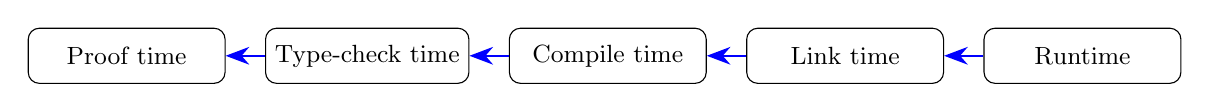
\begin{tikzpicture}[
  node distance=0.5cm,
  every node/.style={draw, rounded corners, minimum width=2.5cm, minimum height=0.7cm, font=\small},
  arrow/.style={-{Stealth[length=3mm]}, thick}
]
  \node (proof) {Proof time};
  \node (typecheck) [right=of proof] {Type-check time};
  \node (compile) [right=of typecheck] {Compile time};
  \node (link) [right=of compile] {Link time};
  \node (runtime) [right=of link] {Runtime};

  \draw[arrow, color=blue] (typecheck) -- (proof);
  \draw[arrow, color=blue] (compile) -- (typecheck);
  \draw[arrow, color=blue] (link) -- (compile);
  \draw[arrow, color=blue] (runtime) -- (link);
\end{tikzpicture}
\end{center}

Each leftward arrow represents a \emph{decision transfer}---moving a decision to an
earlier stage. The axiom asserts that we should transfer decisions as far left as
possible.

\subsection{Proof Time}
Decisions resolved by formal proof, before any type checking begins. Examples include
mathematical lemmas verified by a proof assistant that are then used as axioms in the
type system.

In dependently-typed languages like Agda:
\begin{lstlisting}[language=Haskell, caption={Proof-time decision: commutativity of addition}]
-- This proof is verified once and used as an axiom
plus-comm : (m n : Nat) -> m + n = n + m
plus-comm zero n = sym (plus-zero n)
plus-comm (suc m) n = trans (cong suc (plus-comm m n))
                            (sym (plus-suc n m))
\end{lstlisting}

\subsection{Type-Check Time}
Decisions resolved by the type checker during type inference and checking. This is the
most common target for decision transfer. Examples: type safety, null safety, pattern
exhaustiveness, effect tracking.

\subsection{Compile Time}
Decisions resolved during compilation after type checking. Examples: monomorphization,
constant folding, dead code elimination, inlining.

\subsection{Link Time}
Decisions resolved during linking of separately compiled modules. Examples:
cross-module inlining, whole-program devirtualization, link-time optimization (LTO).

\subsection{Connection to Futamura Projections}

The decision transfer hierarchy is intimately connected to the Futamura projections
from partial evaluation theory.

\begin{definition}[Futamura Projections]
\label{def:futamura}
Let $\mathsf{mix}$ be a partial evaluator. The three Futamura projections are:
\begin{enumerate}[nosep]
  \item $\mathsf{mix}(\mathsf{interp}, \mathsf{source}) = \mathsf{target}$
    \quad(specializing an interpreter yields a compiled program)
  \item $\mathsf{mix}(\mathsf{mix}, \mathsf{interp}) = \mathsf{compiler}$
    \quad(specializing the partial evaluator on an interpreter yields a compiler)
  \item $\mathsf{mix}(\mathsf{mix}, \mathsf{mix}) = \mathsf{cogen}$
    \quad(specializing the partial evaluator on itself yields a compiler generator)
\end{enumerate}
\end{definition}

Each Futamura projection is a decision transfer: it moves decisions from a later stage
(interpretation, compilation, meta-compilation) to an earlier one. The Minimal Runtime
Axiom can be seen as the limiting principle underlying all three projections: transfer
every decision to the earliest possible stage.


% ══════════════════════════════════════════════════════════════════════════
% 9. APPLICATIONS TO LANGUAGE DESIGN
% ══════════════════════════════════════════════════════════════════════════
\section{Applications to Language Design}
\label{sec:language-design}

We now apply the Minimal Runtime Axiom to the design of JAPL (Just Another Programming
Language), a language under development by the YonedaAI Research Collective that
embodies the axiom's principles. JAPL is designed so that each language feature
corresponds to a specific decision transfer.

\subsection{Effect System: Transferring I/O Decisions}

JAPL's algebraic effect system transfers the decision ``what side effects does this
function perform?'' from runtime to type-check time.

\begin{lstlisting}[caption={JAPL effect system as decision transfer}]
effect Database {
  fn query<T: FromRow>(sql: String) -> Result<Vec<T>, DbError>
  fn execute(sql: String) -> Result<u64, DbError>
}

effect Http {
  fn get(url: String) -> Result<Response, HttpError>
  fn post(url: String, body: Body) -> Result<Response, HttpError>
}

// Type signature is the static witness for effect decisions:
fn fetch_user_data(id: UserId) -> Result<UserData, AppError> / {Database, Http} {
  let profile = do Database.query::<Profile>(
    format!("SELECT * FROM profiles WHERE id = {}", id)
  )?;
  let avatar = do Http.get(profile.avatar_url)?;
  Ok(UserData { profile, avatar })
}

// The handler is the compile-time linkage:
fn main() -> Result<(), AppError> / {IO} {
  handle {
    let data = fetch_user_data(UserId(42))?;
    println!("{:?}", data);
    Ok(())
  } with {
    Database => PostgresHandler::new("postgres://localhost/mydb"),
    Http => ReqwestHandler::new(),
  }
}
\end{lstlisting}

\subsection{Ownership System: Transferring Memory Decisions}

JAPL's ownership system, inspired by Rust but extended with linear types and effect
integration, transfers all memory management decisions to compile time.

\begin{lstlisting}[caption={JAPL ownership as decision transfer}]
fn process_stream(stream: Owned<TcpStream>) -> Result<(), NetError> / {IO} {
  let reader = BufReader::new(stream);  // stream moved into reader
  // stream is no longer accessible here (compile-time enforcement)

  for line in reader.lines() {
    let line = line?;
    let parsed: Record = parse(line.as_ref())?;
    process_record(parsed);
  }
  // reader dropped here: TcpStream closed deterministically
  Ok(())
}
\end{lstlisting}

\subsection{Pattern Matching Exhaustiveness: Transferring Dispatch Decisions}

\begin{lstlisting}[caption={Exhaustive pattern matching as decision transfer in JAPL}]
enum Expr {
  Lit(f64),
  Add(Box<Expr>, Box<Expr>),
  Mul(Box<Expr>, Box<Expr>),
  Neg(Box<Expr>),
}

fn eval(expr: Ref<Expr>) -> f64 {
  match expr {
    Expr::Lit(n)       => *n,
    Expr::Add(l, r)    => eval(l) + eval(r),
    Expr::Mul(l, r)    => eval(l) * eval(r),
    Expr::Neg(e)       => -eval(e),
    // Adding a new variant to Expr will cause a compile-time error here
    // until a new match arm is added. No runtime "default" case needed.
  }
}
\end{lstlisting}

\subsection{Type-Derived Serialization: Transferring Wire Format Decisions}

\begin{lstlisting}[caption={Type-derived serialization as decision transfer in JAPL}]
#[derive(Serialize, Deserialize, Schema)]
struct ApiResponse {
  status: u16,
  data: Vec<UserRecord>,
  pagination: PageInfo,
}

// The Schema derivation generates a compile-time wire format.
// No runtime reflection needed for serialization.
// Schema compatibility between services is checked at compile time
// when both services share the type definition.
\end{lstlisting}

\subsection{Supervision Trees: Transferring Failure Policy Decisions}

\begin{lstlisting}[caption={Declarative supervision as decision transfer in JAPL}]
#[supervise(
  strategy = OneForOne,
  max_restarts = 3,
  within = Duration::seconds(60),
)]
struct AppSupervisor {
  #[child(restart = Always)]
  web_server: WebServer,

  #[child(restart = OnFailure)]
  background_worker: Worker,

  #[child(restart = Never)]
  one_shot_migration: Migration,
}

// Failure policy is declared at compile time.
// The supervisor tree structure is type-checked.
// Invalid configurations (e.g., circular supervision) are compile-time errors.
\end{lstlisting}


% ══════════════════════════════════════════════════════════════════════════
% 10. APPLICATIONS TO AGENT ARCHITECTURE
% ══════════════════════════════════════════════════════════════════════════
\section{Applications to Agent Architecture}
\label{sec:agent-arch}

The Minimal Runtime Axiom extends naturally to AI agent systems, where the
compile-time/runtime distinction maps to the design-time/execution-time distinction.
We illustrate through the lens of the ContextFS agent memory architecture and the
AgentHero framework developed at YonedaAI.

\subsection{Agent Capability as a Type}

In agent systems, a critical decision is ``does this agent have the capability to
perform this action?'' In most frameworks, this is checked at runtime. The axiom
suggests typing agent capabilities:

\begin{lstlisting}[caption={Agent capabilities as types in JAPL}]
trait Agent<Caps: CapabilitySet> {
  fn execute<A: Action>(
    self: Ref<Self>,
    action: A,
  ) -> Result<A::Output, AgentError>
  where
    Caps: HasCapability<A::Required>;
    // Compile-time proof that agent has required capabilities
}

struct ResearchAgent;

impl Agent<(WebSearch, FileRead, CodeExec)> for ResearchAgent {
  fn execute<A: Action>(
    self: Ref<Self>,
    action: A,
  ) -> Result<A::Output, AgentError>
  where
    (WebSearch, FileRead, CodeExec): HasCapability<A::Required>
  {
    // If this compiles, the capability check has passed.
    action.run(self)
  }
}
\end{lstlisting}

\subsection{Tool Authorization as a Static Witness}

Tool authorization---deciding whether an agent may invoke a particular tool---is
typically a runtime check against an ACL. With static witnesses:

\begin{lstlisting}[caption={Tool authorization as a static witness}]
type ToolAuth<T: Tool, A: Agent> = proof {
  A::Capabilities: Contains<T::RequiredCapability>
};

fn invoke_tool<T: Tool, A: Agent>(
  agent: Ref<A>,
  tool: T,
  args: T::Args,
  _auth: ToolAuth<T, A>,  // Proof term: must be constructed at compile time
) -> Result<T::Output, ToolError> / {T::Effects} {
  tool.execute(args)
}
\end{lstlisting}

\subsection{Memory Schema as Compile-Time Structure}

In the ContextFS architecture, agent memory is organized by typed schemas. The decision
``is this memory access valid?'' can be transferred to compile time:

\begin{lstlisting}[caption={Typed agent memory in JAPL}]
#[memory_schema]
struct AgentMemory {
  context: TypedStore<ConversationContext>,
  knowledge: TypedStore<KnowledgeGraph>,
  preferences: TypedStore<UserPreferences>,
}

fn recall_context(
  memory: Ref<AgentMemory>,
  query: Query,
) -> Result<Vec<ConversationContext>, MemoryError> / {IO} {
  // Type-safe memory access: cannot accidentally query
  // knowledge store with a context query.
  memory.context.search(query)
}
\end{lstlisting}


% ══════════════════════════════════════════════════════════════════════════
% 11. COMPARISON WITH RELATED FRAMEWORKS
% ══════════════════════════════════════════════════════════════════════════
\section{Comparison with Related Frameworks}
\label{sec:related}

\subsection{Partial Evaluation Theory}

Partial evaluation~\cite{jones1993partial} specializes a program with respect to known
(static) inputs, producing a residual program that depends only on unknown (dynamic)
inputs. The connection to the Minimal Runtime Axiom is direct:

\begin{itemize}[nosep]
  \item Static inputs correspond to $\omega$-independent data
  \item Dynamic inputs correspond to $\omegadata$
  \item The residual program is $\RP$
  \item Binding-time analysis is the identification of $\CP$ vs.\ $\RP$
\end{itemize}

The key difference is that partial evaluation is a \emph{technique} while the Minimal
Runtime Axiom is a \emph{principle}. Partial evaluation transfers decisions from runtime
to compile time via program transformation; the axiom says that \emph{all available}
techniques should be brought to bear, and characterizes the irreducible residual.

\subsection{Multi-Stage Programming}

MetaOCaml~\cite{kiselyov2014metaocaml} and similar systems provide explicit staging
annotations that control when code is generated and executed. The staging certificate
$\sigma$ in our framework corresponds to MetaOCaml's staging levels:

\begin{itemize}[nosep]
  \item Level 0 code (current stage) $\leftrightarrow$ $\sigma$ is trivially satisfied
  \item Level 1 code (next stage) $\leftrightarrow$ $\sigma$ requires future information
  \item Cross-stage persistence $\leftrightarrow$ lifting a witness from an earlier stage
\end{itemize}

MetaOCaml's contribution is making staging \emph{explicit and type-safe}. The axiom
adds the normative principle that staging should be maximized.

\subsection{Dependent Type Theory}

Idris~\cite{brady2013idris}, Agda~\cite{norell2009agda}, and Lean~\cite{demoura2015lean}
represent the state of the art in static witness construction. In these systems, the
type $\tau$ can express arbitrary propositions (by the Curry-Howard correspondence), the
proof term $\pi$ is a program witnessing the proposition, and $\sigma$ is guaranteed
because type checking occurs at compile time.

The Minimal Runtime Axiom adds the observation that even dependent types have a limit:
$\omegadata$ remains irreducibly runtime. Dependent types can \emph{minimize} $\RP$
but cannot eliminate it.

\subsection{Gradual Typing}

Gradual typing~\cite{siek2006gradual} introduces a ``dynamic'' type that defers type
checking to runtime. In the framework of the axiom, gradual typing is a \emph{controlled
Yoneda failure}: the programmer deliberately weakens the Yoneda embedding for specific
types, accepting runtime overhead in exchange for flexibility.

The axiom predicts that gradually typed code will be slower (more runtime decisions) and
less safe (fewer static witnesses) than fully statically typed code, which is empirically
confirmed~\cite{takikawa2016gradual}.

\subsection{Rust's Zero-Cost Abstractions}

Rust~\cite{matsakis2014rust} embodies a practical application of the axiom. Its
``zero-cost abstractions'' principle states that abstractions should compile to code as
efficient as hand-written alternatives. In our framework:
\begin{itemize}[nosep]
  \item Ownership/borrowing: static witnesses for memory decisions
  \item Trait monomorphization: static witnesses for dispatch decisions
  \item \texttt{unsafe}: explicit boundary where static witnesses are unavailable
\end{itemize}

Rust's \texttt{unsafe} keyword is a precise annotation of where the axiom's guarantees
are deliberately suspended---a region where the programmer asserts that the runtime
decisions are justified by concerns the type system cannot capture.


% ══════════════════════════════════════════════════════════════════════════
% 12. THE IMPOSSIBILITY BOUNDARY
% ══════════════════════════════════════════════════════════════════════════
\section{The Impossibility Boundary}
\label{sec:impossibility}

The Minimal Runtime Axiom asserts that runtime should be minimized, but what is the
minimum? This section characterizes the hard boundary beyond which no static analysis
can penetrate.

\begin{theorem}[The $\omega$-Boundary]
\label{thm:omega-boundary}
No static analysis, regardless of expressiveness, can eliminate decisions that depend
on $\omegadata$. Formally, for any type system $T$ (including the Calculus of Inductive
Constructions with arbitrary axiom extensions):
\[
  \RP_{\min} = \{ d \in \DP \mid d \text{ depends on } \omegadata \}
\]
is a lower bound on the runtime set, and this bound is tight.
\end{theorem}

\begin{proof}
The proof proceeds by contradiction. Suppose a decision $d$ depends on $\omegadata$
but has a static witness $\witness = (\tau, \pi, \sigma)$. The staging certificate
$\sigma$ requires that $\pi$ be constructible before execution. But $\pi$ must
establish a proposition about the outcome of $d$, which depends on $\omega$. Since
$\omega$ is not determined before execution (by definition), $\pi$ would need to
determine the indeterminate, a contradiction.

Tightness: for any $d$ not depending on $\omegadata$, we can construct a witness in a
sufficiently expressive system (the proof follows from the completeness of the Calculus
of Inductive Constructions for decidable propositions about finite data).
\end{proof}

\subsection{Connection to the Halting Problem}

The halting problem provides a concrete instance of the $\omega$-boundary within
computation itself.

\begin{theorem}[Halting as $\omega$-Boundary]
\label{thm:halting}
The decision ``does program $Q$ halt on input $x$?'' is at the $\omega$-boundary: it
is $\omega$-dependent when $Q$ or $x$ is not fully known at compile time, and it is
undecidable even when both are known (by Rice's theorem, for non-trivial semantic
properties).
\end{theorem}

\begin{proof}
If $Q$ or $x$ is provided as runtime input (i.e., is part of $\omegadata$), the
halting decision trivially depends on $\omegadata$. If both $Q$ and $x$ are known at
compile time, the question becomes: can the type system decide halting? By Rice's
theorem~\cite{rice1953classes}, no non-trivial semantic property of programs is
decidable. The halting property is a semantic property and is non-trivial. Therefore,
even with full information, the halting decision lies beyond the capability of any
computable static analysis.

Note, however, that \emph{specific instances} of the halting problem can be decided
statically. A type system with termination checking (as in Agda) can prove termination
for many programs. The impossibility is for the \emph{general} case, not for
\emph{all} cases.
\end{proof}

\subsection{Connection to SRIP}

The Self-Reference Incompleteness Principle (SRIP) from YonedaAI's foundational
research~\cite{long2025srip} provides another perspective on the impossibility boundary.
SRIP states that no formal system can fully capture its own semantics---there are always
truths about the system that the system cannot prove.

In the context of the Minimal Runtime Axiom, SRIP implies that a programming language's
type system cannot statically verify all properties of programs written in that language.
There will always be ``G\"{o}del sentences''---program properties that are true but not
provable within the type system---that require runtime verification.

\begin{proposition}[SRIP Bound on $\CP$]
\label{prop:srip}
For any programming language $L$ with type system $T$, there exist programs $P$ in $L$
and decisions $d \in \DP$ that are $\omega$-independent but for which no static witness
$\witness$ can be constructed in $T$. The set of such decisions is non-empty for any
$T$ that is at least as expressive as primitive recursive arithmetic.
\end{proposition}

\begin{proof}
By G\"{o}del's first incompleteness theorem, for any consistent formal system $F$
that can express basic arithmetic, there exists a sentence $G_F$ that is true in the
standard model but not provable in $F$. Encoding $G_F$ as a program property gives a
decision that is $\omega$-independent (it depends only on the program structure) but
lacks a static witness in $T$ (since $T$, viewed as a proof system, cannot prove $G_F$).
\end{proof}

\begin{remark}
The SRIP bound is \emph{theoretical}. In practice, the G\"{o}del sentences of type
systems are exotic and rarely encountered in real programs. The practical impossibility
boundary is almost entirely the $\omega$-boundary, not the SRIP boundary. Nevertheless,
the SRIP bound is important for understanding the \emph{fundamental} limits of static
reasoning.
\end{remark}


% ══════════════════════════════════════════════════════════════════════════
% 13. FORMALIZATION IN CATEGORY THEORY
% ══════════════════════════════════════════════════════════════════════════
\section{Formalization in Category Theory}
\label{sec:category-theory}

We now develop the full categorical formalization of the Minimal Runtime Axiom.

\subsection{The Decision Category}

\begin{definition}[Decision Category]
\label{def:decision-category}
For a program $P$, the \emph{decision category} $\mathcal{D}$ has:
\begin{itemize}[nosep]
  \item \textbf{Objects}: decisions $d \in \DP$
  \item \textbf{Morphisms}: $f : d_1 \to d_2$ exists iff resolving $d_1$ determines (or constrains) $d_2$. Since determination is reflexive, transitive, and antisymmetric (up to equivalence of decisions), $\mathcal{D}$ forms a \emph{preorder}, and in fact a \emph{partial order} when we identify equivalent decisions. This poset structure is essential for the Galois connection underlying the adjunction in \Cref{thm:adjunction}.
  \item \textbf{Composition}: transitive determination (inherited from the preorder)
  \item \textbf{Identity}: each decision trivially determines itself (reflexivity)
\end{itemize}
\end{definition}

\subsection{The Static and Runtime Subcategories}

\begin{definition}[Static and Runtime Subcategories]
\label{def:subcategories}
Given a type system $T$:
\begin{itemize}[nosep]
  \item The \emph{static subcategory} $\mathcal{S}_T \hookrightarrow \mathcal{D}$ is the full subcategory on decisions in $\CP$.
  \item The \emph{runtime subcategory} $\mathcal{R}_T \hookrightarrow \mathcal{D}$ is the full subcategory on decisions in $\RP$.
\end{itemize}
The axiom states: $\mathcal{R}_T$ should be minimal (contain only $\omega$-dependent decisions).
\end{definition}

\subsection{The Axiom as an Adjunction}

\begin{theorem}[The Static-Runtime Adjunction]
\label{thm:adjunction}
There exists an adjunction $F \dashv G$:
\[
  F : \mathcal{R}_T \rightleftarrows \mathcal{S}_T : G
\]
where $F$ (the \emph{static transfer} functor) sends a runtime decision to its
compile-time approximation, and $G$ (the \emph{runtime embedding} functor) sends a
static decision to its runtime execution. The unit $\eta : \id_{\mathcal{R}} \Rightarrow G \circ F$
represents the loss of information when approximating a runtime decision statically, and
the counit $\varepsilon : F \circ G \Rightarrow \id_{\mathcal{S}}$ represents the
elimination of redundant runtime checks after static analysis.
\end{theorem}

\begin{proof}
We construct the adjunction explicitly.

\textbf{The functor $F$}: For each decision $d \in \mathcal{R}_T$, $F(d)$ is the
``best static approximation'' of $d$---the most informative decision in $\mathcal{S}_T$
that constrains $d$. Formally, $F(d) = \bigwedge \{ d' \in \mathcal{S}_T \mid d' \leq d \}$
in the determination order. If no static decision constrains $d$, then $F(d) = \top$
(the trivial decision).

\textbf{The functor $G$}: For each decision $d \in \mathcal{S}_T$, $G(d)$ is the
``runtime execution'' of $d$---the runtime operation that implements what was decided
statically. For a fully static decision, $G(d)$ is a no-op at runtime (the decision
has already been made).

\textbf{Adjunction}: We need to show that
$\mathrm{Hom}_{\mathcal{S}}(F(d_r), d_s) \cong \mathrm{Hom}_{\mathcal{R}}(d_r, G(d_s))$
for all $d_r \in \mathcal{R}_T$ and $d_s \in \mathcal{S}_T$. A morphism $F(d_r) \to d_s$
in $\mathcal{S}_T$ means the best static approximation of $d_r$ determines $d_s$. A
morphism $d_r \to G(d_s)$ in $\mathcal{R}_T$ means the runtime decision $d_r$
determines the runtime execution of $d_s$. These correspond naturally: if the static
approximation determines $d_s$, then the full runtime decision (which refines the
approximation) certainly determines $d_s$'s execution, and conversely.

\textbf{Unit}: $\eta_d : d \to G(F(d))$ maps a runtime decision to the runtime
execution of its static approximation. This is the ``information loss'' of approximation:
$G(F(d))$ is a coarser version of $d$.

\textbf{Counit}: $\varepsilon_d : F(G(d)) \to d$ maps the static approximation of a
runtime-executed static decision back to the original static decision. Since $d$ was
already static, $F(G(d)) = d$, and $\varepsilon$ is the identity.

The triangle identities follow from the fact that $\varepsilon$ is essentially the
identity on static decisions and $\eta$ is injective on runtime decisions.
\end{proof}

\subsection{The Yoneda Embedding as Maximal Static Characterization}

\begin{theorem}[Yoneda Maximality]
\label{thm:yoneda-max}
The Yoneda embedding $\mathsf{y} : \mathcal{C}_T \to [\mathcal{C}_T^{\mathrm{op}}, \Set]$
applied to the type category $\mathcal{C}_T$ provides the \emph{maximal static
characterization} of types: the image of $\mathsf{y}$ captures all and only the
relationships expressible in the type system.
\end{theorem}

\begin{proof}
By the Yoneda lemma, $\mathsf{y}$ is full and faithful. Therefore:
\begin{enumerate}[nosep]
  \item \textbf{Full}: every natural transformation $\Nat(\mathsf{y}(A), \mathsf{y}(B))$
    comes from a morphism $A \to B$ in $\mathcal{C}_T$. This means every ``observable
    relationship'' between types $A$ and $B$ in the presheaf category corresponds to a
    concrete well-typed program.
  \item \textbf{Faithful}: distinct morphisms $f \neq g : A \to B$ in $\mathcal{C}_T$
    give distinct natural transformations. No information is lost.
\end{enumerate}
Maximality follows: any characterization of types that goes beyond $\mathsf{y}$'s image
would require information not expressible as morphisms in $\mathcal{C}_T$---i.e.,
information that the type system cannot express. Such information is precisely the
``epistemic deficit'' of the type system, and accessing it requires runtime inspection
(\Cref{cor:yoneda}).
\end{proof}

\subsection{The Decision Functor}

\begin{definition}[Decision Functor]
\label{def:decision-functor}
The \emph{decision functor} $\mathcal{D}(-) : \mathbf{Lang} \to \Cat$ maps each
programming language (with its type system) to its decision category:
\begin{itemize}[nosep]
  \item On objects: $\mathcal{D}(L)$ is the decision category of all programs in $L$.
  \item On morphisms: a language embedding $L_1 \hookrightarrow L_2$ induces a functor $\mathcal{D}(L_1) \to \mathcal{D}(L_2)$ that preserves static decisions and may transfer runtime decisions to static ones.
\end{itemize}
\end{definition}

\begin{theorem}[Contravariant Runtime Functor]
\label{thm:contravariant}
The runtime functor $\mathcal{R}(-) : \mathbf{Lang}^{\mathrm{op}} \to \Cat$ is
\emph{contravariant}: more expressive languages have smaller runtime categories.
Formally, if $L_1 \hookrightarrow L_2$ (i.e., $L_2$ is at least as expressive as
$L_1$), then there is a functor $\mathcal{R}(L_2) \to \mathcal{R}(L_1)$ that is
generally non-surjective (some runtime decisions in $L_1$ become static in $L_2$).
\end{theorem}

\begin{proof}
By \Cref{prop:monotone}, $\mathcal{C}_{L_1}(P) \subseteq \mathcal{C}_{L_2}(P)$
implies $\mathcal{R}_{L_2}(P) \subseteq \mathcal{R}_{L_1}(P)$. The inclusion
$\mathcal{R}_{L_2}(P) \hookrightarrow \mathcal{R}_{L_1}(P)$ is functorial (it
preserves determination morphisms) and is generally a proper subcategory inclusion.
\end{proof}


% ══════════════════════════════════════════════════════════════════════════
% 14. CONCLUSION
% ══════════════════════════════════════════════════════════════════════════
\section{Conclusion}
\label{sec:conclusion}

We have introduced the \textbf{Minimal Runtime Axiom}: the principle that a decision
reaches runtime if and only if no static witness can be constructed for it. We developed
the formal apparatus of decision spaces, static witnesses $\witness = (\tau, \pi, \sigma)$,
and the three corollaries:

\begin{enumerate}
  \item \textbf{Runtime Irreducibility}: The irreducible runtime core consists exactly of
    $\omega$-dependent decisions---those depending on user input, I/O, time, and
    nondeterminism.
  \item \textbf{The Duality}: The size of the runtime set is proportional to the
    epistemic deficit of the type system, providing a quantitative metric for language
    comparison.
  \item \textbf{The Yoneda Correspondence}: Runtime type inspection is isomorphic to
    failure of the Yoneda embedding, connecting the axiom to the deepest structures of
    category theory.
\end{enumerate}

We showed that the axiom unifies a broad range of existing work---partial evaluation,
multi-stage programming, dependent types, linear types, effect systems---under a single
design principle. We applied it to the design of JAPL, showing how each language feature
corresponds to a specific decision transfer, and extended it to AI agent architecture
where design-time type checking replaces runtime capability checking.

We characterized the impossibility boundary: the $\omega$-boundary imposed by genuinely
unknowable runtime data, and the SRIP boundary imposed by G\"{o}delian incompleteness.
In practice, the $\omega$-boundary dominates, and the goal of language design is to push
all non-$\omega$ decisions to compile time.

The axiom provides language designers with a precise and generative principle:

\begin{quote}
\emph{Every non-$\omega$ decision at runtime is a theorem waiting to be proven.}
\end{quote}

The history of programming languages is the history of proving more and more of these
theorems. The Minimal Runtime Axiom tells us where this history is heading and how to
measure our progress along the way.


% ══════════════════════════════════════════════════════════════════════════
% REFERENCES
% ══════════════════════════════════════════════════════════════════════════
\begin{thebibliography}{99}

\bibitem{milner1978theory}
R.~Milner, ``A theory of type polymorphism in programming,''
\textit{Journal of Computer and System Sciences}, vol.~17, no.~3, pp.~348--375, 1978.

\bibitem{curry1958combinatory}
H.~B.~Curry and R.~Feys, \textit{Combinatory Logic}, vol.~I.
North-Holland, 1958.

\bibitem{howard1980formulae}
W.~A.~Howard, ``The formulae-as-types notion of construction,'' in
\textit{To H.B. Curry: Essays on Combinatory Logic, Lambda Calculus and
Formalism}, pp.~479--490, Academic Press, 1980.

\bibitem{jones1993partial}
N.~D.~Jones, C.~K.~Gomard, and P.~Sestoft, \textit{Partial Evaluation and
Automatic Program Generation}. Prentice Hall, 1993.

\bibitem{futamura1971partial}
Y.~Futamura, ``Partial evaluation of computation process---an approach to a
compiler-compiler,'' \textit{Systems, Computers, Controls}, vol.~2, no.~5,
pp.~45--50, 1971.

\bibitem{kiselyov2014metaocaml}
O.~Kiselyov, ``The design and implementation of BER MetaOCaml,'' in
\textit{Functional and Logic Programming} (FLOPS), Springer, 2014.

\bibitem{davies2001modal}
R.~Davies and F.~Pfenning, ``A modal analysis of staged computation,''
\textit{Journal of the ACM}, vol.~48, no.~3, pp.~555--604, 2001.

\bibitem{brady2013idris}
E.~Brady, ``Idris, a general-purpose dependently typed programming language:
Design and implementation,'' \textit{Journal of Functional Programming},
vol.~23, no.~5, pp.~552--593, 2013.

\bibitem{norell2009agda}
U.~Norell, ``Dependently typed programming in Agda,'' in \textit{Advanced
Functional Programming} (AFP), Springer, 2009.

\bibitem{demoura2015lean}
L.~de~Moura, S.~Kong, J.~Avigad, F.~van~Doorn, and J.~von~Raumer, ``The
Lean theorem prover (system description),'' in \textit{CADE-25}, Springer, 2015.

\bibitem{matsakis2014rust}
N.~D.~Matsakis and F.~S.~Klock~II, ``The Rust language,'' in \textit{ACM
SIGAda Ada Letters}, vol.~34, no.~3, pp.~103--104, 2014.

\bibitem{wadler1989theorems}
P.~Wadler, ``Theorems for free!,'' in \textit{Proceedings of the Fourth
International Conference on Functional Programming Languages and Computer
Architecture} (FPCA), pp.~347--359, ACM, 1989.

\bibitem{reynolds1983types}
J.~C.~Reynolds, ``Types, abstraction and parametric polymorphism,'' in
\textit{Information Processing 83}, pp.~513--523, 1983.

\bibitem{girard1972interpretation}
J.-Y.~Girard, ``Interpr\'{e}tation fonctionnelle et \'{e}limination des
coupures de l'arithm\'{e}tique d'ordre sup\'{e}rieur,'' Ph.D. thesis,
Universit\'{e} Paris VII, 1972.

\bibitem{martinlof1984intuitionistic}
P.~Martin-L\"{o}f, \textit{Intuitionistic Type Theory}. Bibliopolis, 1984.

\bibitem{coquand1988calculus}
T.~Coquand and G.~Huet, ``The calculus of constructions,'' \textit{Information
and Computation}, vol.~76, no.~2-3, pp.~95--120, 1988.

\bibitem{plotkin1977lcf}
G.~D.~Plotkin, ``LCF considered as a programming language,'' \textit{Theoretical
Computer Science}, vol.~5, no.~3, pp.~223--255, 1977.

\bibitem{siek2006gradual}
J.~G.~Siek and W.~Taha, ``Gradual typing for functional languages,'' in
\textit{Scheme and Functional Programming Workshop}, 2006.

\bibitem{takikawa2016gradual}
A.~Takikawa, D.~Feltey, B.~Greenman, M.~S.~New, J.~Vitek, and
M.~Felleisen, ``Is sound gradual typing dead?,'' in \textit{POPL},
pp.~456--468, ACM, 2016.

\bibitem{pierce2002types}
B.~C.~Pierce, \textit{Types and Programming Languages}. MIT Press, 2002.

\bibitem{walker2005substructural}
D.~Walker, ``Substructural type systems,'' in \textit{Advanced Topics in
Types and Programming Languages}, ch.~1, MIT Press, 2005.

\bibitem{honda1993types}
K.~Honda, ``Types for dyadic interaction,'' in \textit{CONCUR}, Springer, 1993.

\bibitem{honda1998language}
K.~Honda, V.~T.~Vasconcelos, and M.~Kubo, ``Language primitives and type
discipline for structured communication-based programming,'' in
\textit{ESOP}, Springer, 1998.

\bibitem{bauer2015programming}
A.~Bauer and M.~Pretnar, ``Programming with algebraic effects and handlers,''
\textit{Journal of Logical and Algebraic Methods in Programming}, vol.~84,
no.~1, pp.~108--123, 2015.

\bibitem{plotkin2009handlers}
G.~Plotkin and M.~Pretnar, ``Handlers of algebraic effects,'' in
\textit{ESOP}, Springer, 2009.

\bibitem{rice1953classes}
H.~G.~Rice, ``Classes of recursively enumerable sets and their decision
problems,'' \textit{Transactions of the American Mathematical Society},
vol.~74, no.~2, pp.~358--366, 1953.

\bibitem{godel1931formal}
K.~G\"{o}del, ``\"{U}ber formal unentscheidbare S\"{a}tze der Principia
Mathematica und verwandter Systeme I,'' \textit{Monatshefte f\"{u}r
Mathematik und Physik}, vol.~38, pp.~173--198, 1931.

\bibitem{maclane1971categories}
S.~Mac~Lane, \textit{Categories for the Working Mathematician}. Springer, 1971.

\bibitem{awodey2010category}
S.~Awodey, \textit{Category Theory}, 2nd~ed. Oxford University Press, 2010.

\bibitem{riehl2017category}
E.~Riehl, \textit{Category Theory in Context}. Dover, 2017.

\bibitem{yoneda1954notion}
N.~Yoneda, ``On the homology theory of modules,'' \textit{Journal of the
Faculty of Science, University of Tokyo}, vol.~7, pp.~193--227, 1954.

\bibitem{long2025srip}
M.~Long, ``The Self-Reference Incompleteness Principle: Fundamental limits of
formal self-knowledge,'' \textit{YonedaAI Research}, 2025.

\bibitem{tait1967intensional}
W.~W.~Tait, ``Intensional interpretations of functionals of finite type I,''
\textit{Journal of Symbolic Logic}, vol.~32, no.~2, pp.~198--212, 1967.

\bibitem{girard1989proofs}
J.-Y.~Girard, Y.~Lafont, and P.~Taylor, \textit{Proofs and Types}.
Cambridge University Press, 1989.

\end{thebibliography}

\end{document}
